\documentclass{beamer}
\usepackage[utf8]{inputenc}

\usetheme{Madrid}
\usecolortheme{default}
\usepackage{amsmath,amssymb,amsfonts,amsthm}
\usepackage{txfonts}
\usepackage{tkz-euclide}
\usepackage{listings}
\usepackage{adjustbox}
\usepackage{array}
\usepackage{tabularx}
\usepackage{gvv}
\usepackage{lmodern}
\usepackage{circuitikz}
\usepackage{tikz}
\usepackage{graphicx}

\setbeamertemplate{page number in head/foot}[totalframenumber]

\usepackage{tcolorbox}
\tcbuselibrary{minted,breakable,xparse,skins}



\definecolor{bg}{gray}{0.95}
\DeclareTCBListing{mintedbox}{O{}m!O{}}{%
  breakable=true,
  listing engine=minted,
  listing only,
  minted language=#2,
  minted style=default,
  minted options={%
    linenos,
    gobble=0,
    breaklines=true,
    breakafter=,,
    fontsize=\small,
    numbersep=8pt,
    #1},
  boxsep=0pt,
  left skip=0pt,
  right skip=0pt,
  left=25pt,
  right=0pt,
  top=3pt,
  bottom=3pt,
  arc=5pt,
  leftrule=0pt,
  rightrule=0pt,
  bottomrule=2pt,
  toprule=2pt,
  colback=bg,
  colframe=orange!70,
  enhanced,
  overlay={%
    \begin{tcbclipinterior}
    \fill[orange!20!white] (frame.south west) rectangle ([xshift=20pt]frame.north west);
    \end{tcbclipinterior}},
  #3,
}
\lstset{
    language=C,
    basicstyle=\ttfamily\small,
    keywordstyle=\color{blue},
    stringstyle=\color{orange},
    commentstyle=\color{green!60!black},
    numbers=left,
    numberstyle=\tiny\color{gray},
    breaklines=true,
    showstringspaces=false,
}
\begin{document}

\title 
{4.7.25}
\date{September 2,2025}


\author 
{Kavin B-EE25BTECH11033}






\frame{\titlepage}
\begin{frame}{Question}
Find the points on the line $x+y=4$ which lie at a unit distance from the line $4x+3y=10$.\\
\end{frame}



\begin{frame}{Theoretical Solution}

According to the question,\\
\begin{align}
    \text{Equation of line $L_1$:}\ \myvec{1&1}\myvec{x\\y}=4
\end{align}
\begin{center}
    $\implies n_1^{\top} \vec{x} = c_1$
\end{center}
and
\begin{align}
    \text{Equation of line $L_2$:}\ \myvec{4&3}\myvec{x\\y}=10
\end{align}
\begin{center}
    $\implies n_2^{\top} \vec{x} = c_2$
\end{center}
\end{frame}

\begin{frame}{Formulae}
The distance $\lambda$ of a vector $\vec{P}$ from the line $\vec{n_2}^{\top}\vec{x}=c_2$ is given by ,
\begin{align}
    \lambda = \frac{\abs{\vec{n_2}^{\top}\vec{P} - c_2}}{\norm{\vec{n_2}}}  
\end{align}
\end{frame}

\begin{frame}{Theoretical Solution}

\begin{align}
    \lambda\norm{\vec{n_2}} = \abs{\vec{n_2}^{\top}\vec{P} - c_2} 
\end{align}
\begin{align}
    \implies\vec{n_2}^{\top}\vec{P} = c_2 \pm \lambda\norm{n_2}
\end{align}
Also, as $\vec{P}$ lies on line $L_1$,
\begin{align}
    \vec{n_1}^{\top}\vec{P} = c_1
\end{align}
On putting eqns $\brak{5}$ and $\brak{6}$ in matrix form we will get,
\begin{align}
    \myvec{n_1 & n_2}^\top\vec{P}=\myvec{c_1\\c_2\pm\lambda\norm{\vec{n_2}}}
\end{align}
where,
\begin{align*}
    \lambda = 1
\end{align*}

\end{frame}


\begin{frame}{Theoretical Solution}
On substituting the values we will get,
\begin{align}
    \myvec{1&1\\4&3}\vec{P}=\myvec{4\\10\pm5}
\end{align}
with the augmented matrix followed by row reduction 
\begin{align}
	R_2 = R_2 - 4 R_1\rightarrow{}\myvec{1&1 &\vrule &  4&\\ 0&-1 & \vrule& -6\pm5&} \\  
	R_2 = -R_2\rightarrow{}\myvec{1&1&\vrule& 4& \\ 0&1 & \vrule &6\mp5} \nonumber \\
	R_1 = R_1-R_2\rightarrow{}\myvec{1&0 & \vrule &-2\pm5&\\ 0&1& \vrule &6\mp5}\nonumber
\end{align}
Therefore the points on $L_1$ which lie at a unit distance from the line $L_2$ are
\begin{align*}
    \vec{P}=\myvec{3\\1} \ \text{and} \ \vec{P}=\myvec{-7\\11}
\end{align*}
\end{frame}

\begin{frame}{Plot}
    \centering
    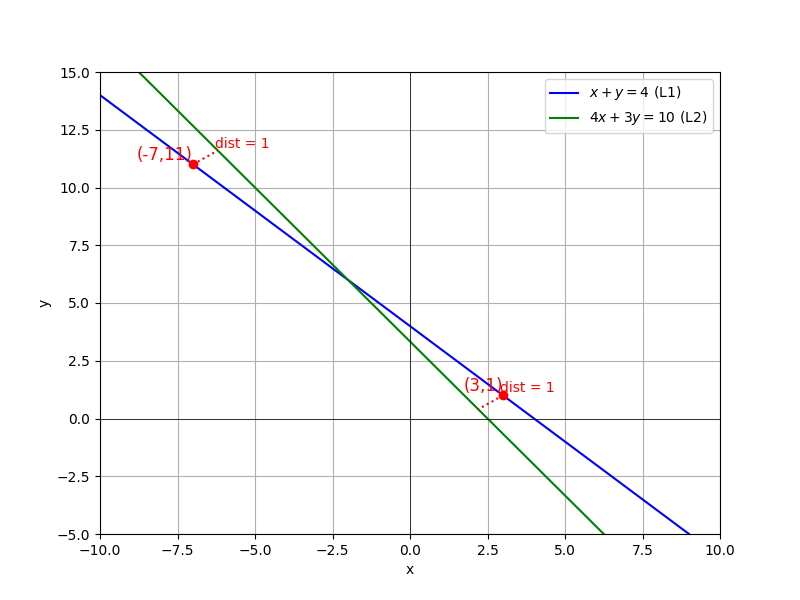
\includegraphics[width=\columnwidth, height=0.8\textheight, keepaspectratio]{figs/fig.png}     
\end{frame}


\end{document}
